\begin{tikzpicture}[xscale=0.75, yscale=1.3, font=\small]
  \draw[<->, gray] (-7,0) -- (7,0) node[right] {$x$};
  \draw[<->, gray] (0,-1.4) -- (0,1.4);
  \draw[thick, dashed, gray, domain=-6.6:6.6, samples=150, smooth] plot (\x, {sin(\x r)});
  \draw[thick, blue, domain=-6.6:6.6, samples=150, smooth] plot (\x, {sin((\x - pi/2) r)});
  \foreach \x/\l in {-6.2832/{-2\pi}, -3.1416/{-\pi}, 3.1416/{\pi}, 6.2832/{2\pi}}
    \draw (\x,0.05) -- (\x,-0.05) node[below=2pt, fill=white, inner sep=1pt] {$\l$};
  \draw (0.08,1) -- (-0.08,1) node[left, fill=white, inner sep=1pt] {$1$};
  \draw (0.08,-1) -- (-0.08,-1) node[left, fill=white, inner sep=1pt] {$-1$};
  \node[blue, right] at (4.2,1.2) {$\sin(x-\tfrac{\pi}{2})$};
  \node[gray, right] at (4.2,-1.25) {$\sin x$ (dashed)};
\end{tikzpicture}
